\chapter{Analisi Lessicale}\label{chap:lexical}
%
\begin{center}

\epsfig{file = cat8.pdf, width = 4cm}
\end{center}
%
L'analisi lessicale scompone un sorgente Kitten in una sequenza di
\emph{token}. Ogni token rappresenta un insieme di stringhe che hanno
lo stesso \emph{ruolo} all'interno del sorgente Kitten. Per esempio, dei token
identificano le parole chiave del linguaggio, un altro gli identificatori, un
altro le costanti
numeriche e \cosi via. Identificare il ruolo delle parole che compongono
un sorgente Kitten \`e essenziale per potere poi ricostruire la struttura
sintattica del codice (Capitolo~\ref{chap:syntactical}).
In questo capitolo vedremo come implementare un analizzatore lessicale
usando degli automi a stati finiti e delle espressioni regolari
e come automatizzare la creazione di un analizzatore lessicale che
riconosce un dato insieme di token, specificato da una lista
di espressioni regolari. Useremo a tal fine il generatore JLex di
analizzatori lessicali, che \`e una versione Java del programma
lex~\cite{Lesk75} inizialmente sviluppato per il linguaggio C.
%
\section{I token Kitten}\label{sec:token_kitten}
%
Abbiamo detto che un token rappresenta un insieme di stringhe. Per esempio,
il token \texttt{THEN} rappresenta l'insieme
di stringhe $\{\mathtt{then}\}$, mentre
il token \texttt{ID} rappresenta l'insieme (potenzialmente infinito) delle
stringhe che sono
\emph{identificatori} Kitten, \cioe nomi di variabili, classi, campi
e metodi. I token che rappresentano \piu di una stringa, come
\texttt{ID}, hanno associato un \emph{valore lessicale}, \cioe
la specifica stringa che essi rappresentano, caso per caso. Si consideri
per esempio la classe \texttt{Led.kit} in Figura~\ref{fig:led}. Il risultato
della sua analisi lessicale \`e in Figura~\ref{fig:led_lexical}.
Si noti come le parole chiave del linguaggio, come \texttt{class},
\texttt{field}, \texttt{void}, \texttt{boolean}, sono rappresentate
da un token specifico. Gli identificatori sono invece rappresentati
dall'unico token \texttt{ID} con associato un valore lessicale, \cioe
la stringa dell'identificatore. Si sarebbe potuto rappresentare anche
le parole chiave come identificatori con associato un valore lessicale.
Per esempio, si poteva usare \texttt{ID(method)} piuttosto che \texttt{METHOD}.
La scelta dei token \`e in parte arbitraria, ma \`e in effetti pensata
per semplificare la successiva ricostruzione della struttura grammaticale
del testo, nella fase di analisi sintattica (Capitolo~\ref{chap:syntactical}).
A quel punto, sar\`a \piu
semplice avere a che fare con \texttt{METHOD} piuttosto che con
\texttt{ID(method)}. Si noti, in Figura~\ref{fig:led_lexical}, come le
parentesi tonde siano rappresentate da due appositi token
(\texttt{LPAREN} ed \texttt{RPAREN}), \cosi come le parentesi
graffe (\texttt{LBRACE} ed \texttt{RBRACE}). Lo stesso accade per le
parentesi quadre (\texttt{LBRACK} ed \texttt{RBRACK}), non mostrate in figura.
Alla fine \`e presente il token fittizio \texttt{EOF} che segnala la fine
del file sorgente. Si noti che spazi, tabulazioni e commenti sono
assenti in Figura~\ref{fig:led_lexical}. Essi vengono infatti scartati
dall'analizzatore lessicale (Sezione~\ref{sec:modes}).

\begin{figure}[t]
\begin{verbatim}
      CLASS from 0 to 4                   ID(this) from 122 to 125
      ID(Led) from 6 to 8                 DOT from 126 to 126
      LBRACE from 10 to 10                ID(state) from 127 to 131
      FIELD from 14 to 18                 ASSIGN from 133 to 134
      BOOLEAN from 20 to 26               FALSE from 136 to 140
      ID(state) from 28 to 32             METHOD from 145 to 150
      CONSTRUCTOR from 37 to 47           BOOLEAN from 152 to 158
      LPAREN from 48 to 48                ID(isOn) from 160 to 163
      RPAREN from 49 to 49                LPAREN from 164 to 164
      LBRACE from 51 to 51                RPAREN from 165 to 165
      RBRACE from 52 to 52                RETURN from 171 to 176
      METHOD from 57 to 62                ID(this) from 178 to 181
      VOID from 64 to 67                  DOT from 182 to 182
      ID(on) from 69 to 70                ID(state) from 183 to 187
      LPAREN from 71 to 71                METHOD from 192 to 197
      RPAREN from 72 to 72                BOOLEAN from 199 to 205
      ID(this) from 78 to 81              ID(isOff) from 207 to 211
      DOT from 82 to 82                   LPAREN from 212 to 212
      ID(state) from 83 to 87             RPAREN from 213 to 213
      ASSIGN from 89 to 90                RETURN from 219 to 224
      TRUE from 92 to 95                  NOT from 226 to 226
      METHOD from 100 to 105              ID(this) from 227 to 230
      VOID from 107 to 110                DOT from 231 to 231
      ID(off) from 112 to 114             ID(state) from 232 to 236
      LPAREN from 115 to 115              RBRACE from 238 to 238
      RPAREN from 116 to 116              EOF from 239 to 239
\end{verbatim}
\caption{Il risultato dell'analisi lessicale della classe in Figura~\ref{fig:led}.}\label{fig:led_lexical}
\end{figure}
%
\section{Token come espressioni regolari}\label{sec:regular_expressions}
%
La specifica dei token di un linguaggio, come Kitten, richiede l'enumerazione
dei token e la descrizione dell'insieme di stringhe che ciascun token
rappresenta. In prima approssimazione,
questi insiemi devono essere disgiunti, in modo che una data
stringa possa appartenere ad al pi\`u un token. La descrizione delle stringhe
rappresentate da un token potrebbe essere fornita in maniera informale, per
esempio in italiano o inglese. Questa scelta avrebbe come conseguenza
negativa la difficile automatizzazione della generazione dell'analizzatore
lessicale, nonch\'e la possibile ambiguit\`a nella specifica dei token.
Decidiamo quindi di usare un linguaggio formale per specificare i token
del linguaggio. Tale linguaggio sar\`a quello delle
\emph{espressioni regolari}.

Un alfabeto specifica l'insieme dei caratteri con cui possiamo comporre
i nostri programmi. Per esempio, potremmo supporre che l'alfabeto di Kitten
siano i caratteri presenti sulla tastiera del calcolatore, o l'insieme dei
caratteri unicode.
%
\begin{definition}[Alfabeto]\label{def:alphabet}
Un \emph{alfabeto} $\Lambda$ \`e un insieme finito di elementi, detti
\emph{caratteri}.
\end{definition}
%
\noindent
Un'espressione regolare \`e un elemento del seguente insieme, costruito
a partire da un alfabeto.
%
\begin{definition}[Espressione Regolare]\label{def:regular_expression}
L'insieme delle \emph{espressioni regolari} su un alfabeto
$\Lambda$ \`e il pi\`u piccolo insieme $\mathcal{R}$ tale che
%
\begin{itemize}
\item $\emptyset\in\mathcal{R}$ (l'insieme vuoto \`e un'espressione regolare)
\item $\varepsilon\in\mathcal{R}$ (la stringa vuota \`e un'espressione
      regolare)
\item $\Lambda\subseteq\mathcal{R}$ (ogni carattere \`e un'espressione
      regolare)
\item se $r_1,r_2\in\mathcal{R}$ allora $r_1r_2\in\mathcal{R}$
      (l'insieme delle espressioni regolari \`e chiuso per \emph{sequenza} o
      \emph{concatenazione})
\item se $r_1,r_2\in\mathcal{R}$ allora $r_1|r_2\in\mathcal{R}$
      (l'insieme delle espressioni regolari \`e chiuso per \emph{alternanza})
\item se $r\in\mathcal{R}$ allora $r^*\in\mathcal{R}$
      (l'insieme delle espressioni regolari \`e chiuso per \emph{iterazione}).
\end{itemize}
\end{definition}
%
Se, per esempio, $\Lambda=\{\mathtt{a},\mathtt{b},\mathtt{c}\}$, allora
$\mathtt{a}\in\mathcal{R}$, ma anche $\mathtt{abc}\in\mathcal{R}$, nonch\'e
$\mathtt{a|b|abc}\in\mathcal{R}$ ed $\mathtt{ab}^*\in\mathcal{R}$.
Assumeremo di potere usare delle parentesi tonde nelle espressioni
regolari, al fine di chiarire la loro struttura sintattica.
Per esempio, scriveremo $\mathtt{a|b|(abc)}$ per distingure tale espressione
regolare da $\mathtt{(a|b|a)bc}$ e scriveremo $\mathtt{(ab)}^*$ per distinguere
tale espressione regolare da $\mathtt{a(b^*)}$. Assumeremo che $*$ abbia
massima priorit\`a, per cui, in assenza di parentesi,
$\mathtt{ab^*}$ va inteso come $\mathtt{a(b^*)}$.
Va comunque osservato che le parentesi non fanno strettamente parte del
linguaggio delle espressioni regolari, ma servono solo a evidenziare la
struttura della loro definizione induttiva. Ecco perch\'e le parentesi
non figurano nella Definizione~\ref{def:regular_expression}.

Definita la \emph{sintassi} delle espressioni regolari,
passiamo a definire la loro
\emph{semantica}. Dal momento che i token rappresentano insiemi di stringhe
e che vogliamo usare le espressioni regolari per specificare i token,
sembra sensato che la semantica o significato di una espressione regolare sia
un insieme di stringhe, ovvero un \emph{linguaggio}.
%
\begin{definition}[Linguaggio]\label{def:language}
Un \emph{linguaggio} su un alfabeto $\Lambda$ \`e un qualsiasi sottoinsieme
delle stringhe finite ottenibili a partire dai caratteri di $\Lambda$.
Tale insieme di stringhe \`e tradizionalmente indicato come $\Lambda^*$.
\end{definition}
%
Per esempio, l'insieme $\{\mathtt{then}\}$ \e un linguaggio sull'alfabeto
inglese, formato da un'unica stringa. L'insieme $\{\mathtt{a},\mathtt{aa},
\mathtt{aaa},\ldots\}$ \`e un linguaggio sull'alfabeto $\{\mathtt{a},
\mathtt{b}\}$ formato da tutte e sole le stringhe formate da una o pi\`u
$\mathtt{a}$. Si noti che $\emptyset$ \`e un linguaggio su qualsiasi
alfabeto, formato dall'insieme finito di stringhe. Anche
$\{\varepsilon\}$ \`e un linguaggio su qualsiasi alfabeto, formato dalla
stringa vuota. Si noti che $\emptyset\not=\{\varepsilon\}$.
%
\begin{definition}[Linguaggio di un'Espressione Regolare]
  \label{def:regular_language}
Data un'espressione regolare $r$ sull'alfabeto $\Lambda$, la sua
\emph{semantica} $\mathcal{L}(r)$ \`e il linguaggio su $\Lambda$ definito
tramite le seguenti regole:
%
\begin{itemize}
\item $\mathcal{L}(\emptyset)=\emptyset$
\item $\mathcal{L}(\varepsilon)=\{\varepsilon\}$
\item $\mathcal{L}(a)=\{a\}$ per ogni $a\in\Lambda$
\item $\mathcal{L}(r_1r_2)=\{s_1s_2\mid s_1\in\mathcal{L}(r_1)\text{ ed }
      s_2\in\mathcal{L}(r_2)\}$
\item $\mathcal{L}(r_1|r_2)=\mathcal{L}(r_1)\cup\mathcal{L}(r_2)$
\item $\mathcal{L}(r^*)=\{s_1\cdots s_n\mid n\ge 0\text{ ed }s_i\in
      \mathcal{L}(r)\text{ per ogni }0\le i\le n\}$.
\end{itemize}
\end{definition}
%
\noindent
Si noti che nella semantica di $\mathcal{L}(r^*)$ si ammette che
$n=0$, nel qual caso $s_1\cdots s_n=\varepsilon$. Concludiamo che
$\varepsilon\in\mathcal{L}(r^*)$ per ogni espressione regolare $r$.

Diremo spesso
che $\mathcal{L}(r)$ \`e il linguaggio \emph{denotato} dall'espressione
regolare $r$ o, pi\`u semplicemente, il \emph{linguaggio dell'espressione $r$}.

Si consideri per esempio l'espressione regolare $\mathtt{then}$ sull'alfabeto
inglese. Essa denota il linguaggio
%
\[
  \mathcal{L}(\mathtt{then})=\{s_1s_2s_3s_4\mid s_1\in\mathcal{L}(\mathtt{t}),
    \ s_2\in\mathcal{L}(\mathtt{h}),\ s_3\in\mathcal{L}(\mathtt{e})
    \text{ ed }s_4\in\mathcal{L}(\mathtt{n})\}
    =\{\mathtt{then}\}.
\]
L'espressione regolare $\mathtt{aa^*}$ denota il linguaggio
\begin{align*}
  \mathcal{L}(\mathtt{aa^*})&=\{s_1s_2\mid s_1\in\mathcal{L}(\mathtt{a})
    \text{ ed }s_2\in\mathcal{L}(\mathtt{a^*})\}\\
  &=\{s_1s_2\mid s_1\in\{\mathtt{a}\}\text{ ed }
    s_2=\underbrace{\mathtt{a\cdots a}}_n\text{ con }n\ge 0\}\\
  &=\{\underbrace{\mathtt{a\cdots a}}_n\mid n\ge 1\}.
\end{align*}
%
Possiamo similmente definire l'espressione regolare
che denota l'insieme degli \emph{identificatori},
cio\`e delle sequenze non vuote
di caratteri alfabetici, come $\alpha\alpha^*$, dove $\alpha=\mathtt
{a|b|c|d|\cdots|w|x|y|z}$. Si noti che i linguaggi di programmazione, come
Kitten, usano una definizione pi\`u complessa di \emph{identificatore}:
una sequenza non vuota di caratteri, minuscoli o maiuscoli, di cifre e del
carattere $\_$, che cominci per\`o con un carattere alfabetico. Per poter
definire tale nozione di identificatore, usiamo delle \emph{abbreviazioni}.
%
\begin{definition}[Abbreviazioni]\label{def:abridged}
Le seguenti sintassi sono abbreviazioni delle corrispondenti espressioni
regolari:
%
\begin{itemize}
\item $\alpha\mathtt{?}$ \`e un'abbreviazione per $\alpha|\varepsilon$
\item $\alpha^+$ \`e un'abbreviazione per $\alpha\alpha^*$
\item se l'alfabeto \`e totalmente ordinato, allora $\mathtt{[a-z]}$ \`e
      un'abbreviazione per $\mathtt{a|b|c|\cdots|x|y|z}$ dove
      $\mathtt{b|c|\cdots|x|y}$ \`e l'insieme dei caratteri compresi
      fra $\mathtt{a}$ e $\mathtt{z}$. Questa abbreviazione viene estesa
      a intervalli multipli, come in $\mathtt{[a-zA-Z]}$.
\end{itemize}
%
A questo punto possiamo definire gli identificatori come il linguaggio denotato
dall'espressione regolare
%
\[
  \mathtt{ID}=\mathtt{[a-zA-Z][a-zA-Z0-9\_]^*}
\]
%
\end{definition}
%
Compreso il linguaggio delle espressioni regolari, possiamo immaginare di
specificare i token di un linguaggio di programmazione con un insieme di
espressioni regolari, ognuna etichettata con il token che essa rappresenta.
Ci sono per\`o delle problematiche inerenti a questa semplice idea:
%
\begin{description}
\item[\textit{Coincidenza pi\`u lunga}.]
  Pu\`o accadere che la stessa stringa sia
  riconoscibile come un unico token o come due token consecutivi. Per esempio,
  la stringa $\mathtt{ciao}$ pu\`o essere riconosciuta come un'istanza del
  token $\mathtt{ID}$ per gli identificari ma anche come due istanze contigue
  del token $\mathtt{ID}$: l'identificatore $\mathtt{ci}$ seguito
  dall'identificatore
  $\mathtt{ao}$. Al fine di risolvere questa ambiguit\`a, decidiamo di
  preferire la prima interpretazione, ovvero di inglobare quanti pi\`u
  caratteri possibile a un token, prima di passare al prossimo.
  Conseguentemente, $\mathtt{ciao}$ \`e un singolo token identificatore.
  Questa scelta si chiama \emph{coincidenza pi\`u lunga} o
  \emph{longest match}.
\item[\textit{Priorit\`a delle regole}.]
  Non deve accadere che una stringa abbia due o pi\`u espressioni
  regolari che possano denotarla. In tal caso, infatti, non \`e chiaro
  quale delle due espressioni regolari, ovvero token, debba essere associata
  alla stringa. Si pu\`o richiedere che le espressioni regolari nella nostra
  enumerazione dei token denotino insiemi disgiunti. Questa richiesta \`e
  per\`o irrealistica, perch\'e comporta l'uso di espressioni regolari
  molto complesse. Per esempio, l'espressione $\mathtt{ID}$ per gli
  identificatori
  denota anche delle parole chiave del linguaggio, come $\mathtt{then}$, che
  noi vorremmo invece denotare con un'espressione regolare, o token, specifica.
  Definire un'espressione regolare alternativa a $\mathtt{ID}$ che denoti tutti
  gli identificatori che non siano parole chiave \`e possibile ma molto
  complicato. \`E molto pi\`u semplice, invece, dire che, nella nostra
  enumerazione delle espressioni regolari, quelle che
  figurano prima hanno priorit\`a su quelle che figurano dopo. A questo punto,
  \`e sufficiente inserire le espressioni regolari per le parole chiave
  prima di $\mathtt{ID}$, per dare alle prime priorit\`a su $\mathtt{ID}$.
\end{description}

Vediamo adesso come automatizzare la costruzione di un analizzatore
lessicale a partire da una specifica dei token del linguaggio data come
un'enumerazione di espressioni regolari.
%
\section{La generazione dell'analizzatore lessicale}\label{sec:jlex}
%
Per rappresentare un token, usiamo la classe in
Figura~\ref{fig:java_cup.runtime.Symbol}, che fa parte
del programma \texttt{JavaCup} che \`e un generatore di analizzatori
sintattici. Il motivo per cui usiamo tale classe \`e che \cosi
facendo sar\`a \piu semplice interfacciare il nostro analizzatore lessicale
con l'analizzatore sintattico che costruiremo nel
Capitolo~\ref{chap:syntactical}, dal momento
che entrambi utilizzano la stessa struttura dati per rappresentare i token.
%
\begin{figure}
\begin{verbatim}
    public class Symbol {
      public int sym;       // il codice che identifica il token
      public int left;      // il carattere a cui inizia
      public int right;     // il carattere a cui finisce
      public Object value;  // il valore lessicale associato, se esiste
      ...
    }
\end{verbatim}
\caption{La classe \texttt{java\_cup.runtime.Symbol.java}, che rappresenta
un token Kitten.}\label{fig:java_cup.runtime.Symbol}
\end{figure}
%
I codici \texttt{sym} dei token sono enumerati dentro la classe
\texttt{syntactical/sym.java}. Anche tale file fa parte del generatore di
analizzatori sintattici in modo che sia l'analizzatore lessicale
che quello sintattico usano gli stessi codici per i token
(si veda anche la Sezione~\ref{sec:java_cup}).
La Figura~\ref{fig:java_cup.runtime.Symbol} mostra che di ogni token \`e
possibile conoscere la posizione \texttt{left} a cui inizia,
espressa in numero di caratteri dall'inizio del file, commenti inclusi,
la posizione \texttt{right} a cui finisce e l'eventuale
valore lessicale \texttt{value}, se \`e definito per quel tipo di token.
Per esempio, il token \texttt{ID(Led)} in
Figura~\ref{fig:led_lexical} ha \texttt{left} pari a $6$, \texttt{right} pari
ad $8$ e \texttt{value} legato alla stringa \texttt{Led}. I token
che non hanno valore lessicale avranno \texttt{value} pari a \texttt{null}.

Quello che vogliamo ottenere \`e un analizzatore lessicale per i token Kitten.
Al posto di generare tutta la sequenza di token, come quella in
Figura~\ref{fig:led_lexical}, e poi passarla all'analizzatore sintattico,
\`e molto \piu economico generare un token alla volta e passarlo
all'analizzatore sintattico. Anche quest'ultimo per\`o
dovr\`a essere capace di lavorare con un token alla volta.
L'interfaccia dell'analizzatore lessicale sar\`a quindi quella
mostrata in Figura~\ref{fig:lexer}.
%
\begin{figure}
\begin{center}
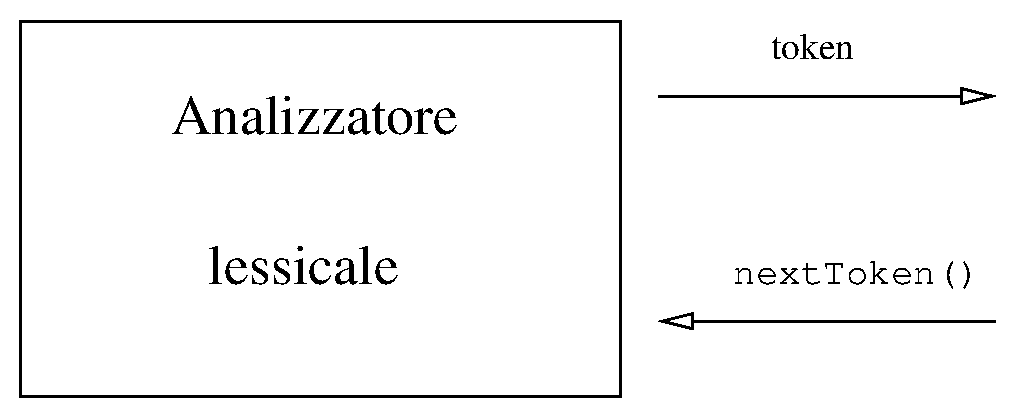
\epsfig{file = lexer.eps, width = 6cm}
\end{center}
\caption{L'interfaccia dell'analizzatore lessicale.}\label{fig:lexer}
\end{figure}
%
Il metodo \texttt{nextToken()} restituisce un token alla volta.

Genereremo l'analizzatore lessicale per Kitten in modo automatico, a partire
dalla specifica dei token che deve riconoscere. A tal fine useremo un
programma Java di nome JLex. La Figura~\ref{fig:jlex} mostra il
modo in cui generiamo l'analizzatore lessicale usando JLex.
%
\begin{figure}
\begin{center}
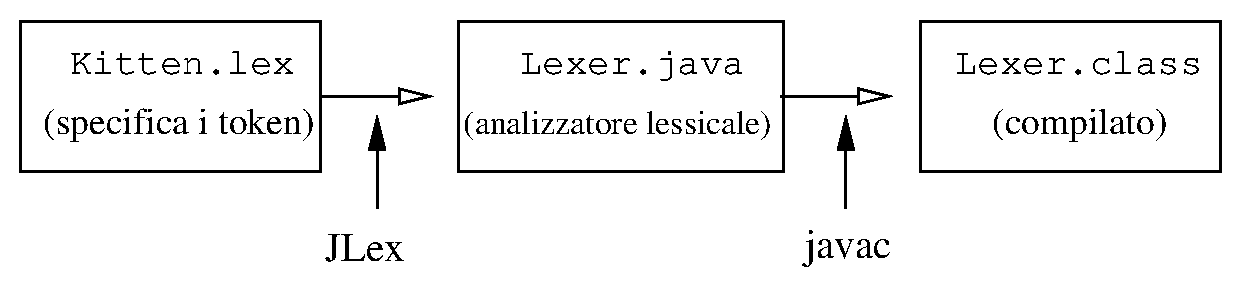
\epsfig{file = jlex.eps, width = \textwidth}
\end{center}
\caption{La generazione dell'analizzatore lessicale per Kitten.}
  \label{fig:jlex}
\end{figure}
%
Dentro al file \texttt{lexical/Kitten.lex} enumeriamo
le espressioni regolari che denotano i token del linguaggio
Kitten, in una sintassi comprensibile dal programma JLex.
Per ogni espressione regolare va fornito, nel file
\texttt{lexical/Kitten.lex}, un pezzo di codice
Java che viene eseguito quando viene riconosciuto il token corrispondente.
Normalmente tale codice Java non fa altro
che sintetizzare il token opportuno (\cioe un oggetto della classe
\texttt{java\_cup.runtime.Symbol} in Figura~\ref{fig:java_cup.runtime.Symbol})
e restituirlo.

Fornendo al programma JLex la specifica
\texttt{lexical/Kitten.lex} dei token, otteniamo un programma Java
di nome \texttt{lexical/Lexer.java} che pu\`o essere compilato
come un qualsiasi programma Java. Tale programma \`e l'analizzatore
lessicale. Il nome \texttt{nextToken} della funzione che vogliamo generare
(Figura~\ref{fig:lexer}) viene specificato scrivendo la sua specifica dentro
\texttt{lexical/Kitten.lex}:
%
\begin{verbatim}
%function nextToken
%type java_cup.runtime.Symbol
\end{verbatim}
%
con \texttt{\%type} abbiamo specificato il suo tipo di ritorno.

Programmi generati in maniera automatica, come \texttt{lexical/Lexer.java},
sono normalmente di difficile lettura per un essere umano.
Fidiamoci quindi del risultato, e descriviamo invece in \piu dettagli
il contenuto del file \texttt{lexical/Kitten.lex}.
%
\section{La specifica dei token}\label{sec:token_specification}
%
Abbiamo detto che il file \texttt{lexical/Kitten.lex} contiene la
descrizione dei token Kitten, sotto forma di espressioni regolari con
associata un'azione di
sintesi del token corrispondente. Per esempio esso contiene le
seguenti coppie espressione regolare/azione:
%
\begin{verbatim}
  <YYINITIAL>while        {return tok(sym.WHILE, null);}
  <YYINITIAL>for          {return tok(sym.FOR, null);}
  ....
  <YYINITIAL>"+"          {return tok(sym.PLUS, null);}
  <YYINITIAL>"-"          {return tok(sym.MINUS, null);}
  <YYINITIAL>"*"          {return tok(sym.TIMES, null);}
  <YYINITIAL>"/"          {return tok(sym.DIVIDE, null);}
  <YYINITIAL>"="          {return tok(sym.EQ, null);}
  <YYINITIAL>"!="         {return tok(sym.NEQ, null);}
  <YYINITIAL>"<"          {return tok(sym.LT, null);}
  <YYINITIAL>"<="         {return tok(sym.LE, null);}
  ....
  <YYINITIAL>":="         {return tok(sym.ASSIGN, null);}
  ....
\end{verbatim}
%
che riconoscono rispettivamente
le parole chiave \texttt{while}, \texttt{for}, il segno di addizione ecc.
La sintassi \texttt{while} \`e un'espressione regolare che va intesa
come $\mathtt{w}\cdot\mathtt{h}\cdot\mathtt{i}\cdot\mathtt{l}\cdot\mathtt{e}$,
\cioe come la concatenazione sequenziale di cinque caratteri. La notazione
\texttt{<YYINITIAL>} specifica che queste regole sono attive quando
l'analizzatore lessicale \e nella \emph{modalit\`a} di default
\texttt{YYINITIAL}.
Parleremo \piu tardi delle modalit\`a (Sezione~\ref{sec:modes}).
Per adesso ci basta sapere che, all'inizio, l'analizzatore lessicale \e
in modalit\`a \texttt{YYINITIAL}, per cui le regole precedenti sono attive.
L'azione corrispondente a ciascuna regola, che viene eseguita quando
il token corrispondente \`e stato riconosciuto, \`e fra parentesi graffe.
Si tratta di codice Java. Per adesso, esso sintetizza il token
corrispondente alle espressioni regolari, usando l'identificatore
numerico unico di ciascun token
(per esempio, \texttt{sym.WHILE}) e \texttt{null} come valore
lessicale. Il metodo \texttt{tok} non fa altro che costruire un oggetto
della classe in Figura~\ref{fig:java_cup.runtime.Symbol}:
%
\begin{verbatim}
private java_cup.runtime.Symbol tok(int kind, Object value) {
  return new java_cup.runtime.Symbol
    (kind,yychar,yychar + yylength(),value);
}
\end{verbatim}
%
La variabile \texttt{yychar} contiene il numero di caratteri tra l'inizio del
file e l'inizio del token. Il metodo \texttt{yylength()} ritorna
la lunghezza del token riconosciuto.
Metodi di ausilio, come quello precedente, sono inseriti in
\texttt{lexical/Kitten.lex} fra i delimitatori \verb!%{! e
\verb!}%! e vengono ricopiati testualmente da JLex dentro
\texttt{lexical/Lexer.java}.

I token che hanno un valore lessicale sono specificati in maniera appena \piu
complicata:
%
\begin{verbatim}
<YYINITIAL>[a-zA-Z][a-zA-Z0-9_]*
    {return tok(sym.ID,yytext());}
<YYINITIAL>[0-9]+
    {return tok(sym.INTEGER,new Integer(yytext()));}
<YYINITIAL>[0-9]*"."[0-9]+
    {return tok(sym.FLOATING,new Float(yytext()));}
\end{verbatim}
%
Si noti come il valore lessicale degli identificatori \texttt{ID} sia
la stringa che rappresenta l'identificatore, mentre per interi e numeri
a virgola mobile si tratta, rispettivamente,
di un oggetto di classe \texttt{java.lang.Integer} e \texttt{java.lang.Float}.
Il programma JLex accorda maggiore priorit\`a alle regole
specificate prima in \texttt{lexical/Kitten.lex}. Al fine, per esempio, di non
fare riconoscere la parola chiave \texttt{while} come un
identificatore, occorre mettere la regola per il \texttt{while}
prima di quella per gli identificatori (Sezione~\ref{sec:regular_expressions}).

Esiste infine una regola che riconosce qualsiasi carattere ma che, essendo
messa alla fine, viene eseguita solo quando nessun'altra regola
\`e applicabile. Tale regola segnala un'errore lessicale, \cioe
la lettura di un carattere che non \e associabile ad alcun token:
%
\begin{verbatim}
  <YYINITIAL>.            {errorMsg.error(yychar,"Unmatched input");}
\end{verbatim}
%
Il carattere \texttt{.} (punto) \`e un'espressione regolare che denota
l'insieme dei caratteri dell'alfabeto. La si pu\`o immaginare come
un'abbreviazione dell'alternanza fra tutti i caratteri dell'alfabeto.
%
\javatip{
Se si dovessero aggiungere nuovi token all'enumerazione contenuta nel file
\texttt{lexical/Kitten.lex}, occorre fare attenzione alla posizione in
cui le loro espressioni regolari vengono inserite. Molti studenti tendono
a inserire queste nuove espressioni regolari in fondo, dopo la regola
che usa il carattere punto. Questa \`e la peggior scelta che si pu\`o
fare: se il token \`e formato da un unico carattere, esso non verr\`a
mai riconosciuto perch\'e la regola col punto avr\`a priorit\`a sulla nuova
regola (Sezione~\ref{sec:regular_expressions}).
Se il token \`e formato da pi\`u caratteri alfabetici, esso non
verr\`a mai riconosciuto perch\'e la regola per l'identificatore avr\`a
priorit\`a sulla nuova regola. \`E quindi consigliabile inserire le
espressioni regolari per nuovi token subito dopo l'enumerazione della
punteggiatura, prima degli identificatori.}
%
\section{La segnalazione di errori}\label{sec:errors}
%
Abbiamo appena visto che l'analizzatore lessicale pu\`o avere bisogno
di segnalare un errore all'utente di Kitten. Lo stesso (e molto \piu
spesso) accadr\`a con l'analizzatore sintattico e con quello semantico.
Tutti questi analizzatori usano la stessa classe
\texttt{errorMsg/ErrorMsg.java} per segnalare
errori. La sua interfaccia\footnote{
Per \piu informazioni sulle classi e i metodi di Kitten, ricordiamo
che \`e disponibile la documentazione JavaDoc dentro la
directory \texttt{javadocs} della distribuzione di Kitten.}
\e in Figura~\ref{fig:errorMsg.ErrorMsg}.
%
\begin{figure}[t]
\begin{verbatim}
public class ErrorMsg {
  /* costruttore: si chiede il nome del file che si sta compilando */
  public ErrorMsg(String fileName) { ... }

  /* chiamata quando si incontra un newline in fileName */
  public newline(int pos) { ... }

  /* segnala un errore msg alla posizione pos dall'inizio di fileName */
  public error(int pos, String msg) { ... }

  /* dice se si e' verificato almeno un errore */
  public static boolean anyErrors() { ... }
}
\end{verbatim}
\caption{La classe \texttt{errorMsg.ErrorMsg.java} per la segnalazione di errori.}\label{fig:errorMsg.ErrorMsg}
\end{figure}
%
Il metodo \texttt{error()} segnala un errore all'utente. La posizione
dell'errore \e indicata all'utente con la notazione \texttt{riga:colonna}.
Ma il metodo \texttt{error()} richiede solo il numero \texttt{pos}
di caratteri passati dall'inizio del file che si sta compilando.
Per potere trasformare \texttt{pos} in \texttt{riga:colonna}, occorre
che l'oggetto di segnalazione di errori sia al corrente di dove, nel
file sorgente, si trovano i caratteri di newline. Ecco perch\'e, ogni volta
che si incontra tale carattere, l'analizzatore lessicale chiama il
metodo \texttt{newline()}:
%
\begin{verbatim}
  <YYINITIAL>\n           {errorMsg.newline(yychar);}
\end{verbatim}
%
Si noti che questa regola ha anche l'effetto secondario di
scartare il carattere newline, \poiche non vogliamo
i caratteri di spaziatura nel risultato dell'analisi lessicale
(Figura~\ref{fig:led_lexical}). Conoscendo le posizioni dei caratteri
di newline, \`e possibile sapere quanti newline occorrono nei primi
\texttt{pos} caratteri del file sorgente ed \`e quindi possibile
recuperare l'informazione di \texttt{riga}. La \texttt{colonna}
sar\`a il numero di caratteri tra l'ultimo newline e \texttt{pos}.

Il campo \texttt{errorMsg} dell'analizzatore lessicale
contiene la sua struttura di segnalazione di errore.
Essa \`e creata dal costruttore di
quest'ultimo a partire dal nome del file che si sta compilando.
%
\section{JLex: da espressioni regolari ad automi finiti non deterministici}
  \label{sec:nfa}
%
Abbiamo visto che JLex trasforma una sequenza di espressioni regolari
in un programma Java (l'analizzatore lessicale)
capace di riconoscere i token denotati da tali
espressioni regolari. Vediamo adesso di capire come funziona questo programma.

Le espressioni regolari sono degli ottimi strumenti per \emph{descrivere}
un insieme di stringhe, il loro linguaggio, ma certamente non per
\emph{riconoscere} tale insieme: data una stringa, vogliamo sapere se
appartiene o meno al linguaggio generato da una data espressione regolare.
Al fine di riconoscere un linguaggio, useremo degli \emph{automi a stati
finiti}, che ammettono anche una semplice implementazione tramite un
calcolatore.
%
\begin{definition}[Automa Finito non Deterministico]\label{def:nfa}
Un \emph{automa finito non deterministico} su un alfabeto $\Lambda$ \`e un
grafo orientato finito i cui nodi sono detti \emph{stati} e i cui archi, detti
\emph{transizioni}, sono etichettati con un carattere in $\Lambda$ o con
$\varepsilon$. Un nodo del grafo \`e identificato come \emph{iniziale}
e un insieme di nodi del grafo come \emph{finali}.
\end{definition}
%
\begin{figure}[t]
\begin{center}
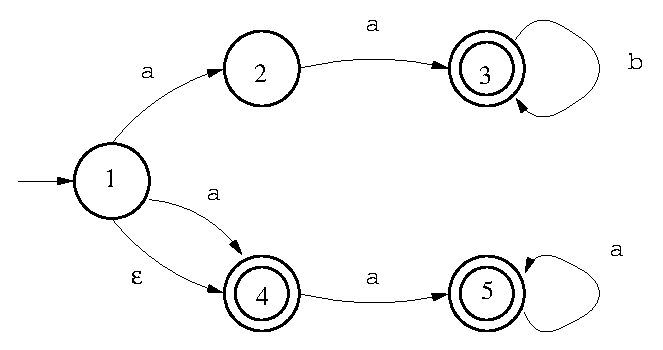
\epsfig{file = nfa.eps, width = 8cm}
\end{center}
\caption{Un automa finito non deterministico.}\label{fig:nfa}
\end{figure}
%
\noindent
La Figura~\ref{fig:nfa} mostra un automa finito non deterministico
sul linguaggio $\Lambda=\{\mathtt{a},\mathtt{b}\}$. Il nodo iniziale
\`e individuato da una freccia entrante. I nodi finali sono individuati
con una doppia cerchiatura.

Un \emph{percorso} in un automa \`e una sequenza di nodi legati da archi.
%
\begin{definition}[Percorso]\label{def:path}
Un \emph{percorso} in un automa finito non deterministico \`e una sequenza
di nodi $n_1\to^{c_1}n_2\to^{c_2}\cdots\to^{c_{k-1}}n_k$
tale che per ogni $i=1,\ldots,k-1$ esiste un arco $n_i\to^{c_i}n_{i+1}$
fra $n_i$ ed $n_{i+1}$. La \emph{stringa espressa} da un
percorso \`e la concatenazione delle etichette sugli archi che passano per i
nodi del percorso, cio\`e $c_1c_2\cdots c_{k-1}$.
\end{definition} 
%
\noindent
Per esempio, l'automa in Figura~\ref{fig:nfa} possiede un percorso
$4\to^\mathtt{a}5\to^\mathtt{a}5\to^\mathtt{a}5$ che esprime la stringa
\texttt{aaa}. Possiamo quindi definire il linguaggio \emph{accettato} da un
automa come l'insieme delle stringhe espresse da un percorso dell'automa
che comincia nel suo unico nodo iniziale e termina in un nodo finale.
%
\begin{definition}[Linguaggio Accettato da un Automa]\label{def:nfa_accept}
Il linguaggio $\mathcal{L}(A)$ \emph{accettato} da un automa non deterministico
$A$ \`e
\[
  \mathcal{L}(A)=\left\{s\in\Lambda^*\left|\begin{array}{l}
    s=c_1\cdots c_{k-1}\text{ ed esiste un percorso }n_1\to^{c_1}\cdots
      \to^{c_{k-1}}n_k\text{ di $A$}\\
    \text{tale che $n_1$ \`e il nodo iniziale di $A$ ed
          $n_k$ \`e un nodo finale di $A$}
  \end{array}\right.\right\}.
\]
\end{definition}
%
\noindent
Per esempio, possiamo determinare il linguaggio accettato dall'automa in
Figura~\ref{fig:nfa} considerando l'unione dei linguaggi accettati in ciascuno
dei suoi tre stati di accettazione. Essa \`e il linguaggio
fatto dalle stringhe che cominciano con due \texttt{a} e continuano con
un numero arbitrario (anche nullo) di \texttt{b}, dalle stringhe che
cominciano con una o due \texttt{a}
e continuano con un numero arbitrario (anche nullo)
di \texttt{a}, e dalla stringa vuota. Si noti che un automa pu\`o
accettare una stringa tramite vari percorsi differenti. Per esempio,
l'automa in Figura~\ref{fig:nfa} accetta la stringa \texttt{a} tramite
il percorso $1\to^\mathtt{a}4$ ma anche tramite il percorso
$1\to^\varepsilon 4\to^\mathtt{a}5$.

Il linguaggio accettato dall'automa in Figura~\ref{fig:nfa} \`e in effetti
quello denotato dall'espressione regolare $\varepsilon\mathtt{|aab^*
|aa^*|aaa^*}$ (che sarebbe possibile semplificare in $\mathtt{aab^*|a^*}$).
Questa non \`e una coincidenza: si pu\`o in effetti dimostrare
che, dato un linguaggio, esiste un automa finito non deterministico che
lo accetta se e solo se esiste un'espressione regolare che lo denota. Di questo
risultato vediamo adesso solo come \`e possibile costruire un automa finito non
deterministico a partire da una espressione regolare, in modo che quest'ultima
denoti lo stesso linguaggio accettato dall'automa. Pi\`u in dettaglio,
forniamo una definizione induttiva di un automa finito non deterministico
\emph{indotto} da una data espressione regolare.

Procediamo per induzione sulla struttura delle espressioni regolari, definendo
un automa non deterministico corrispondente a ciascun tipo di espressione
regolare della Definizione~\ref{def:regular_expression}. In questa costruzione
manterremo l'invariante che l'automa costruito avr\`a sempre
\emph{al pi\`u uno stato di accettazione}.

L'espressione regolare $\emptyset$ denota il linguaggio vuoto
(Definizione~\ref{def:regular_language}). Un automa che accetta lo
stesso linguaggio \`e il seguente:
%
\begin{center}
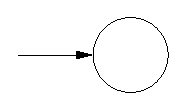
\epsfig{file = empty_nfa.eps, width = 3cm}
\end{center}
%
Esso non ha stati di accettazione e conseguentemente accetta
l'insieme vuoto di stringhe.

L'espressione regolare $\varepsilon$ denota un linguaggio che contiene la
sola stringa $\varepsilon$. Esso \`e lo stesso linguaggio accettato dall'automa
%
\begin{center}

\epsfig{file = epsilon_nfa.eps, width = 3cm}
\end{center}
%
Si noti che lo stato iniziale e quello di accettazione di questo automa
coincidono.

L'espressione regolare $a$, con $a\in\Lambda$, denota un linguaggio formato
dalla sola stringa $a$. Esso \`e lo stesso linguaggio accettato dall'automa
%
\begin{center}
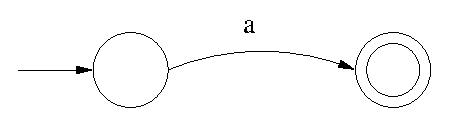
\epsfig{file = a_nfa.eps, width = 8cm}
\end{center}

L'espressione regolare $r_1r_2$, cio\`e la sequenza di due espressioni regolari
$r_1$ ed $r_2$, denota il linguaggio formato dalle stringhe ottenute
concatenando una stringa del linguaggio denotato da $r_1$ con una stringa
del linguaggio denotato da $r_2$. Otteniamo quindi un automa che accetta lo
stesso linguaggio concatenando sequenzialmente l'automa corrispondente ad
$r_1$ con l'automa corrispondente ad $r_2$:
%
\begin{center}
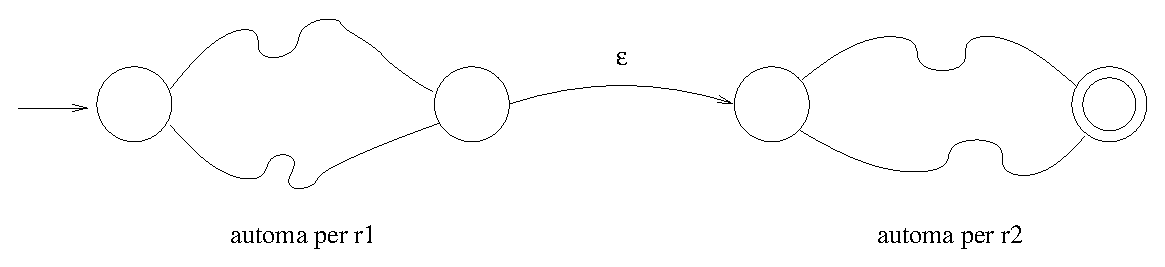
\epsfig{file = r1r2.eps, width = 15cm}
\end{center}
%
Si noti che lo stato di accettazione dell'automa corrispondente ad $r_1$
non \`e pi\`u di accettazione nell'automa composto per $r_1r_2$. Se inoltre
$r_1$ non ha stati di accettazione, allora la transizione etichettata con
$\varepsilon$ non viene aggiunta.

L'espressione regolare $r_1|r_2$ denota l'unione dei linguaggi di
$r_1$ e di $r_2$. Otteniamo quindi un automa che accetta lo stesso
linguaggio mettendo in alternativa gli automi corrispondenti alle
espressioni regolari $r_1$ ed $r_2$:
%
\begin{center}
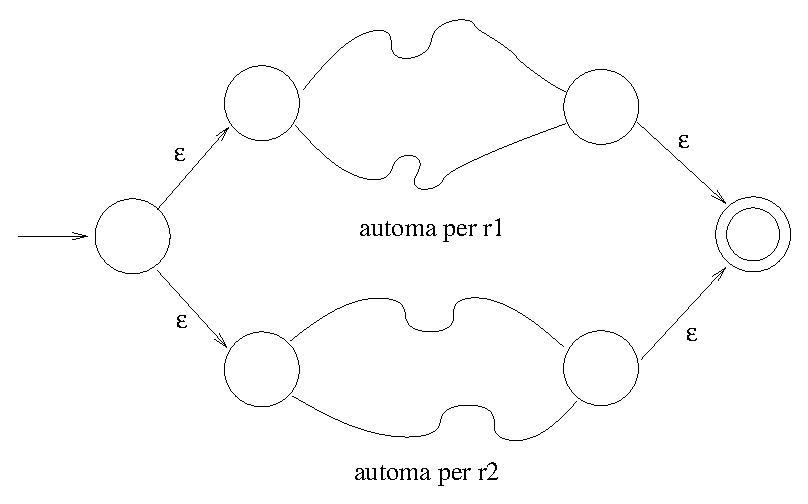
\epsfig{file = r1orr2.eps, width = 13cm}
\end{center}
%
Si noti che gli stati di accettazione degli automi corrispondenti ad $r_1$
ed $r_2$ non sono pi\`u di accettazione nell'automa composto per $r_1|r_2$,
mentre un nuovo stato di accettazione \`e stato aggiunto in quest'ultimo.
Se inoltre gli automi per $r_1$ o $r_2$ non hanno stati di accettazione
allora non si aggiunge la freccia (o le frecce) etichettate con
$\varepsilon$ che portano nello stato di accettazione.

L'espressione regolare $r^*$ denota il linguaggio ottenuto ripetendo un
numero arbitrario di volte le stringhe del linguaggio denotato da $r$.
Otteniamo un automa che accetta lo stesso linguaggio creando un ciclo
sull'automa corrispondente ad $r$. Questo ciclo pu\`o essere percorso
un numero arbitrario di volte, eventualmente anche nessuna volta:
%
\begin{center}
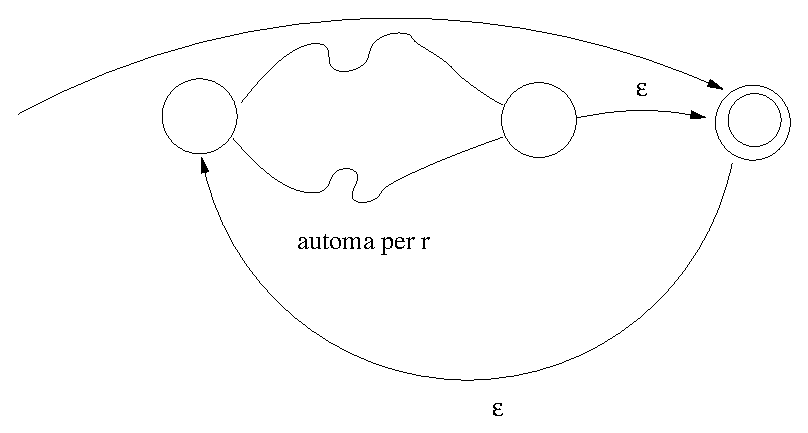
\epsfig{file = rstar.eps, width = 13cm}
\end{center}
%
Si noti che lo stato di accettazione dell'automa per $r$ non \`e pi\`u
di accettazione nell'automa per $r^*$, e che in quest'ultimo lo stato
finale e quello iniziale coincidono. Se inoltre l'automa corrispondente
ad $r$ non avesse alcuno stato di accettazione, non si mette la transizione
etichettata con $\varepsilon$ che porta nello stato di accettazione.

Si consideri per esempio l'espressione regolare
$\mathtt{\varepsilon|aab^*|aa^*|aaa^*}$. Abbiamo gi\`a notato
che essa denota lo stesso linguaggio riconosciuto dall'automa
in Figura~\ref{fig:nfa}. Il risultato della costruzione esplicita di un automa
corrispondente a tale espressione regolare, usando le regole induttive di
costruzione che abbiamo appena descritto, \`e mostrato in
Figura~\ref{fig:nfa_built}.
%
\begin{figure}[t]
\begin{center}
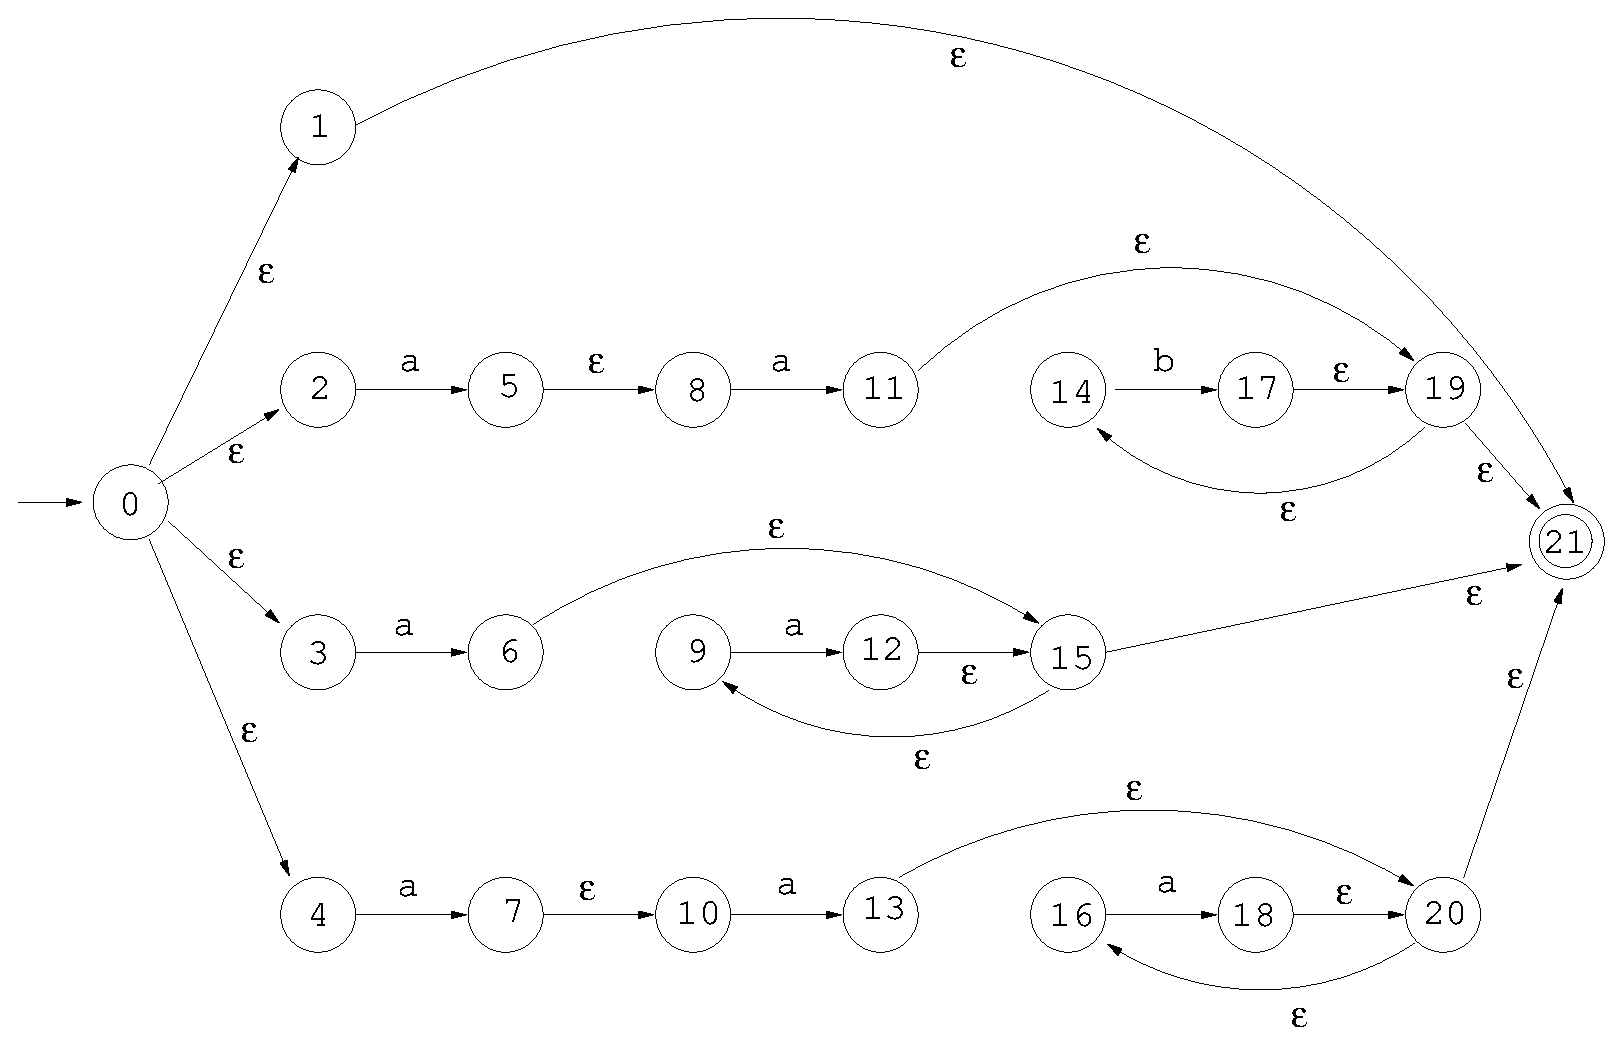
\epsfig{file = nfa_built.eps, width = 15cm}
\end{center}
\caption{Un automa finito non deterministico costruito induttivamente a partire dall'espressione regolare $\mathtt{\varepsilon|aab^*|aa^*|aaa^*}$. La numerazione dei nodi \`e arbitraria.}\label{fig:nfa_built}
\end{figure}
%
L'automa in Figura~\ref{fig:nfa_built} \`e diverso da quello in
Figura~\ref{fig:nfa}. In particolare, esso contiene \piu stati e transizioni.
I due automi sono per\`o \emph{equivalenti}, nel senso che essi
accettano lo stesso linguaggio (Definizione~\ref{def:nfa_accept}).
%
\section{JLex:
 da automi finiti non deterministici ad automi finiti deterministici}
  \label{sec:dfa}
%
La nozione di \emph{automa} che abbiamo dato nella Definizione~\ref{def:nfa}
caratterizza automi finiti \emph{non deterministici} in quanto \`e
possibile che ci siano \piu transizioni uscenti da uno stesso stato etichettate
con lo stesso carattere dell'alfabeto o transizioni etichettate con
$\varepsilon$. Se quindi tali automi sono utili
per \emph{descrivere} un linguaggio, essi sono per\`o scomodi per
\emph{riconoscere} un linguaggio, cio\`e per fornire una procedura effettiva
che permetta di determinare se una stringa appartiene o meno al linguaggio
che essi denotano. Occorrerebbe infatti a tal fine considerare tutti
i percorsi possibili nell'automa.

Se limitassimo ad al \piu uno il numero delle transizioni uscenti da uno
stesso stato etichettate con un dato carattere e vietassimo
delle transizioni etichettate con $\varepsilon$, otterremmo un tipo di automa
che ci permette di riconoscere se una stringa appartiene al linguaggio che
esso denota semplicemente cercando l'\emph{unico} percorso nell'automa
per tale stringa, se esiste. Questo nuovo tipo di automa \`e detto
\emph{deterministico}.
%
\begin{definition}[Automa Finito Deterministico]\label{def:dfa}
Un \emph{automa finito deterministico} \`e un automa finito
non deterministico senza transizioni etichettate con $\varepsilon$
e tale che per ciascun nodo e ciascun carattere
dell'alfabeto c'\`e al \piu una transizione
uscente dal nodo etichettata con tale carattere.
\end{definition}
%
\noindent
Per esempio, l'automa in Figura~\ref{fig:nfa} sarebbe deterministico se non
ci fosse la transizione etichettata con $\varepsilon$ e se le due
transizioni uscenti dal nodo $1$ ed etichettate con \texttt{a} avessero
etichette diverse.

Dal momento che un automa finito deterministico \`e un caso particolare
di automa finito non deterministico, le definizioni di \emph{percorso}
(Definizione~\ref{def:path}) e di \emph{linguaggio accettato}
(Definizione~\ref{def:nfa_accept}) sono valide anche per gli automi finiti
deterministici. \`E quindi immediato osservare che se un linguaggio \`e
accettato da un automa deterministico allora esso \`e accettato anche da un
automa non deterministico (lo stesso automa!). Il viceversa \`e anch'esso
vero, bench\'e meno immediato da dimostrare e intuitivamente meno ovvio.
In effetti \`e possibile simulare un automa finito non deterministico
con un automa deterministico i cui stati \emph{rappresentano} insiemi di
stati dell'automa non deterministico simulato. Questo significa che il
non determinismo non aggiunge potenza espressiva agli automi a stati finiti.

La trasformazione di un automa non deterministico in uno deterministico
comporta la definizione della \emph{$\varepsilon$-chiusura}
e della \emph{transizione su un carattere} di un insieme di stati.
%
\begin{definition}[$\varepsilon$-chiusura e transizione su un carattere]
  \label{def:closure}
Dato un automa finito non deterministico $A$ e un insieme $N$ dei suoi nodi,
la \emph{$\varepsilon$-chiusura} $\varepsilon(N)$ di $N$ \`e l'insieme $N$
stesso unito all'insieme dei nodi raggiungibili da un nodo di
$N$ usando solo transizioni etichettate con $\varepsilon$:
\[
  \varepsilon(N)=\{n'\in A\mid\text{esiste $n\in N$ tale che
                   $n\to^\varepsilon\cdots\to^\varepsilon n'$}\}.
\]
Se $c\in\Lambda$, la \emph{transizione su $c$ di $N$}, indicata come
$c(N)$, \`e l'insieme dei
nodi di $A$ raggiungibili da un nodo di $N$ tramite una transizione
etichettata con $c$ seguita da un numero arbitrario di transizioni
etichettate con $\varepsilon$:
\[
  c(N)=\varepsilon(\{n'\mid\text{esiste }n\in N\text{ tale che }
                   n\to^c n'\}).
\]
\end{definition}
%
\noindent
Per esempio, in Figura~\ref{fig:nfa_built} abbiamo
\begin{align*}
  \varepsilon(\{0\})&=\{0,1,2,3,4,21\}\\
  \varepsilon(\{5,8\})&=\{5,8\}\\
  \texttt{a}(\{0,1,2,3,4,21\})&=\{5,6,7,8,9,10,15,21\}\\
  \texttt{b}(\{0,1,2,3,4,21\})&=\emptyset.
\end{align*}

\`E possibile trasformare un automa finito non deterministico $A$ in uno
deterministico $A'$ equivalente i cui stati sono insiemi di stati di $A$.
Lo stato iniziale di $A'$ e $\varepsilon(i)$, dove $i$ \`e lo stato iniziale
di $A$. Da ogni stato $s$ di $A'$ e per ogni carettere $c$ dell'alfabeto,
esce da $s$ una transizione etichettata con $c$ che porta nello
stato $c(s)$ di $A'$. Se $c(s)=\emptyset$ allora si pu\`o fare a meno di
indicare la transizione. Gli stati di accettazione di $A'$ sono quelli che
contengono almeno uno degli stati di accettazione di $A$.
Per esempio, l'automa finito non deterministico in Figura~\ref{fig:nfa_built}
viene trasformato in quello deterministico mostrato in
Figura~\ref{fig:dfa_built}. Si noti che tutti i suoi stati sono di
accettazione.
%
\begin{figure}[t]
\begin{center}
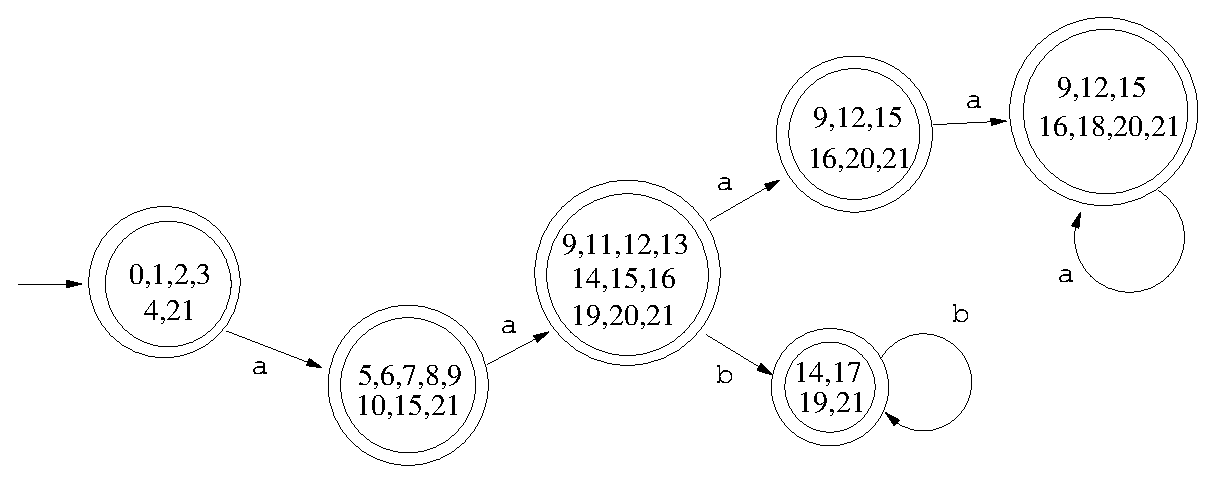
\epsfig{file = dfa_built.eps, width = 15cm}
\end{center}
\caption{Un automa finito deterministico ottenuto dall'automa non deterministico in Figura~\ref{fig:nfa_built}.}\label{fig:dfa_built}
\end{figure}

La trasformazione da espressione regolare ad automa della Sezione~\ref{sec:nfa}
fornisce in genere un automa finito \emph{non deterministico} a causa
delle regole di traduzione dell'alternanza di due espressioni regolari.
Tale automa pu\`o poi essere trasformato in un automa finito deterministico
equivalente con la trasformazione appena descritta. Questo \`e proprio
quello che fa JLex, ottenendo un automa deterministico che pu\`o
essere \piu comodamente eseguito su una macchina sequenziale.
Va detto comunque che, per una maggiore efficienza, JLex
evita di costruire l'automa non deterministico ma costruisce invece
direttamente quello deterministico. Si tratta comunque di una ottimizzazione
della trasformazione fin qui descritta.

In genere l'automa ottenuto eliminando il
non determinismo potrebbe essere \emph{ridondante}, nel senso che
esso pu\`o contenere due stati con identiche funzioni, che possono quindi
venire fusi in un unico stato. Questo \`e per
esempio il caso degli stati $\{9,12,15,16,20,21\}$ e
$\{9,12,15,16,18,20,21\}$ in Figura~\ref{fig:dfa_built}. Essi potrebbero essere
fusi in un unico stato con una transizione uscente per \texttt{a} che porta
sullo stato stesso, riducendo il numero di stati dell'automa.
L'\emph{ottimizzazione} del numero di stati dell'automa deterministico
risultante dalla trasformazione viene quindi effettuata da JLex
al fine di ridurre la dimensione dell'automa deterministico finale.
Quest'ultimo viene infine scritto nel file \texttt{Lexer.java}
(Figura~\ref{fig:jlex}) sotto forma di un sorgente Java che contiene
l'insieme dei nodi e la tabella di transizione dell'automa.

Occorre adesso comprendere l'ultimo aspetto del funzionamento di JLex.
Esso infatti permette di riconoscere un \emph{insieme} di token e non una
sola espressione regolare. Inoltre esso implementa, fra tali token,
i meccanismi di coincidenza \piu lunga e priorit\`a delle regole
descritti nella Sezione~\ref{sec:regular_expressions}.
Consideriamo questi aspetti nella sezione seguente.
%
\section{JLex: la costruzione di un automa non deterministico per un insieme di token}\label{sec:jlex_for_tokens}
%
In Sezione~\ref{sec:nfa} abbiamo visto come un'espressione regolare pu\`o
essere trasformata in un automa finito non deterministico che accetta lo
stesso linguaggio denotato dall'espressione regolare. In Sezione~\ref{sec:dfa}
abbiamo visto poi come tale automa possa venire trasformato in un automa
equivalente ma deterministico e quindi di \piu facile implementazione su una
macchina sequenziale. In questa sezione vediamo come JLex applica
queste tecniche per riconoscere un insieme di token.

JLex costruisce l'automa finito non deterministico corrispondente
all'espressione regolare che denota ciascun token, usando la tecnica
descritta nella Sezione~\ref{sec:nfa}. Tali automi vengono poi
messi in alternanza creando un unico, grande automa avente uno stato
iniziale legato agli stati iniziali di ciascun automa. Per esempio, per
i due token
%
\begin{verbatim}
  IF     if
  ID     [a-z][a-z]*
\end{verbatim}
%
il programma JLex costruisce l'automa
in Figura~\ref{fig:nfa_if_id}. Abbiamo etichettato alcune transizioni
con un intervallo di caratteri, il cui senso \`e che esse rappresentano in
effetti un \emph{insieme} di transizioni, una per ciascun carattere
nell'intervallo. Si noti inoltre che abbiamo annotato, accanto a
ciascuno stato di accettazione, qual \`e il token accettato in tale stato.
%
\begin{figure}[t]
\begin{center}
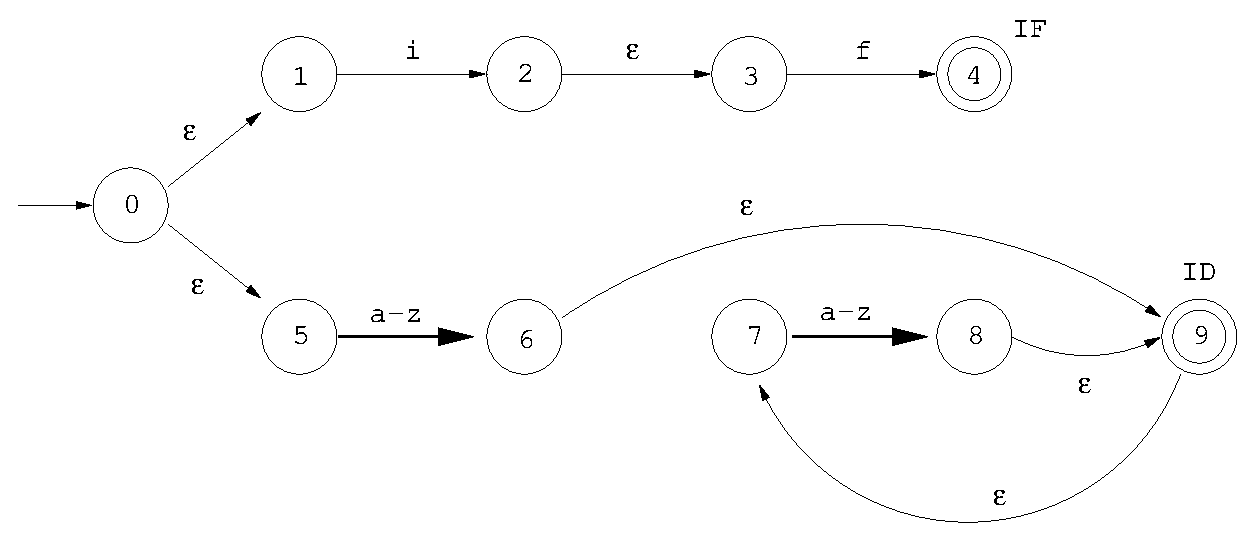
\epsfig{file = nfa_if_id.eps, width = 15cm}
\end{center}
\caption{Un automa finito non deterministico per i token \texttt{IF} ed \texttt{ID}.}\label{fig:nfa_if_id}
\end{figure}
%
JLex trasforma quindi tale automa in un automa finito deterministico,
con la tecnica descritta nella Sezione~\ref{sec:dfa}. Il risultato, per il
nostro esempio, \`e mostrato in Figura~\ref{fig:dfa_if_id}.
\`E possibile che uno stesso stato dell'automa deterministico venga etichettato
con \piu token, poich\'e contiene lo stato finale di \piu sotto-automi.
Questo \`e il caso dello stato etichettato con \texttt{IF} ed \texttt{ID}
in Figura~\ref{fig:dfa_if_id}. Questo significa che se si arriva in tale stato
allora i caratteri letti dall'inizio del file possono essere considerati sia
come un'istanza del token \texttt{ID} che come un'istanza del token
\texttt{IF}. Abbiamo gi\`a visto come si risolve questa ambiguit\`a:
dando precedenza al token che figura prima nell'enumerazione
(Sezione~\ref{sec:regular_expressions}).
Nel nostro caso, il token \texttt{IF} \`e stato enumerato per prima e
quindi l'etichetta \texttt{ID} viene rimossa e in tale stato si riconosce
solo il token \texttt{IF}.

Il risultato dell'elaborazione effettuata da JLex \`e quindi
un automa come quello in Figura~\ref{fig:dfa_if_id}, scritto in Java.
Ogni volta che si chiama il metodo \texttt{nextToken()}, tale automa viene
eseguito a partire dalla posizione corrente nel file sorgente. Quando occorre
fermarsi in questa lettura? Ci si potrebbe fermare non appena si finisce in uno
stato di accettazione. Ma questo significherebbe che \texttt{abc} verrebbe
riconosciuto come tre token \texttt{ID} piuttosto che come un unico token
\texttt{ID}. JLex decide quindi di avanzare nel file di input
finch\'e esiste una transizione possibile nell'automa. Quando non esiste
\piu alcuna transizione possibile, si restituisce il token che etichettava
l'ultimo stato di accettazione per cui si \`e passati.
Questo modo di procedere implementa quindi la \emph{coincidenza \piu
lunga} della Sezione~\ref{sec:regular_expressions}. Se nessuno stato di
accettazione \`e stato ancora incontrato, JLex
d\`a un messaggio di errore. Si noti comunque che quest'ultima situazione
\`e comunque impossibile nel caso di Kitten poich\'e nella enumerazione dei
token abbiamo inserito una regola di default che accetta qualsiasi carattere
(Sezione~\ref{sec:token_specification}).

L'implementazione dell'automa da parte di JLex deve tener conto di
un ultimo problema: i caratteri letti dopo l'ultimo stato di accettazione
per cui si \`e passati vanno \emph{rimessi} nel file di input per essere
processati alla prossima richiesta di \texttt{nextToken()}. A tal fine
basta utilizzare due puntatori nel file di input: uno che punta all'ultimo
stato di accettazione per cui si \`e passati e uno che punta all'ultimo
carattere letto. Prima di terminare una chiamata a \texttt{nextToken()},
JLex ha cura di riportare l'ultimo puntatore a coincidere col primo.
%
\begin{figure}[t]
\begin{center}
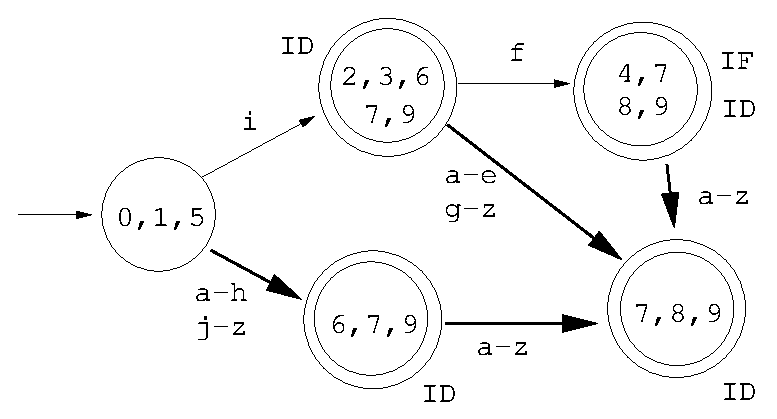
\epsfig{file = dfa_if_id.eps, width = 12cm}
\end{center}
\caption{L'automa finito deterministico costruito a partire dall'automa non deterministico in Figura~\ref{fig:nfa_if_id}.}\label{fig:dfa_if_id}
\end{figure}
%
\section{Modalit\`a lessicali: commenti e stringhe}\label{sec:modes}
%
Le regole contenute in \texttt{lexical/Kitten.lex} hanno come
prefisso una \emph{modalit\`a} che indica quando esse sono attive. Normalmente,
l'analizzatore lessicale \`e nella modalit\`a di default \texttt{YYINITIAL}.
\`E possibile per\`o cambiare modalit\`a tramite il metodo
\texttt{yybegin()}. Occorre per prima cosa dichiarare le nuove modalit\`a
dentro \texttt{lexical/Kitten.lex}:
%
\begin{verbatim}
  %state COMMENT
  %state STRING
\end{verbatim}
%
La scelta di queste due modalit\`a \`e finalizzata a semplificare la
gestione di commenti e stringhe. Per esempio,
la modalit\`a \texttt{COMMENT} si attiva quando incontriamo la sequenza
di caratteri \texttt{/*}:
%
\begin{verbatim}
  <YYINITIAL>"/*"         {commentCount++; yybegin(COMMENT);}
\end{verbatim}
%
La variabile \texttt{commentCount} conta il livello di annidamento
dei commenti visti fino a questo momento. Essa \e dichiarata fra i
delimitatori \verb!%{! e \verb!%}! e inizializzata a $0$.

Le uniche regole attive in modalit\`a \texttt{COMMENT} hanno come scopo
di scartare tutti i caratteri letti fino alla chiusura dell'ultimo
commento, tenendo conto dell'annidamento. Non dobbiamo per\`o dimenticare
di registrare le posizioni dei caratteri di newline:
%
\begin{verbatim}
  <COMMENT>"*/"           {commentCount--;
                           if (commentCount == 0) yybegin(YYINITIAL);}
  <COMMENT>"/*"           {commentCount++;}
  <COMMENT>\n             {newline();}
  <COMMENT>.              {}
\end{verbatim}

Occorre evitare che il file sorgente termini con un commento
ancora aperto. A tal fine usiamo il fatto che,
quando l'analizzatore lessicale giunge alla fine del file sorgente,
viene eseguito il codice specificato, dentro \texttt{lexical/Kitten.lex},
fra i delimitatori \texttt{\%eofval\{} e \texttt{\%eofval\}}. Nel nostro
caso abbiamo scelto di eseguire quanto segue:
%
\begin{verbatim}
  %eofval{
          {
            if (commentCount != 0) err("Unclosed comment");
            return tok(sym.EOF, null);
          }
  %eofval}
\end{verbatim}
%
ovvero controlliamo che il file non termini con un commento ancora aperto e
poi restituiamo comunque il token fittizio \texttt{EOF}.

La modalit\`a \texttt{STRING} si attiva quando si incontra
un carattere di doppio apice. Essa riconosce la stringa fra doppi apici e
processa le sequenze di escape. Memorizza il valore lessicale dentro una
variabile \texttt{myString} che viene usata come valore lessicale del
token \texttt{STRING}:
%
\begin{verbatim}
  <YYINITIAL>"\"" {myString = ""; yybegin(STRING);}
  <STRING>\\n     {myString += "\n";}
  <STRING>\\t     {myString += "\t";}
  ... altre sequenze di escape ...
  <STRING>"\""    {yybegin(YYINITIAL); return tok(sym.STRING,myString);}
  <STRING>\n      {errorMsg.newline(yychar); myString += "\n";}
  <STRING>.       {myString += yytext();}
\end{verbatim}
%
La seconda e la terza regola inseriscono un carattere di escape
dentro la stringa quando viene riconosciuto la corrispondente
espressione di escape dentro il file sorgente. Si noti che l'espressione
regolare \verb!\\n! \`e formata da \emph{due} caratteri \verb!\\! e \texttt{n}.
Il primo \`e a sua volta una sequenza di escape di JLex per
esprimere il carattere \verb!\!. Esistono altre espressioni di escape
per inserire, per esempio, un carattere a partire dal suo codice ASCII.
Esse sono esaminabili dentro \texttt{lexical/Kitten.lex}.
La terz'ultima regola riporta l'analizzatore in modalit\`a \texttt{YYINITIAL}
quando si incontra il carattere doppio apice di chiusura della stringa.
Le ultime due regole accumulano tutti caratteri dentro \texttt{myString}.
%
\greycomment{
L'uso di comandi Java con memoria, come l'assegnamento su \texttt{commentCount}
e \texttt{myString}, ha l'effetto di aumentare la potenza di JLex,
al punto che si potrebbe pensare di affidargli compiti molto \piu
complessi dell'analisi lessicale. Per esempio, la stessa analisi sintattica
(Capitolo~\ref{chap:syntactical})
potrebbe essere effettuata all'interno di JLex.
In effetti, l'uso di variabili Java d\`a a JLex la
capacit\`a di superare il potere espressivo limitato delle espressioni
regolari o degli automi a stati finiti, per accedere all'espressivit\`a
superiore di sistemi di riconoscimento di linguaggi basati su una quantit\`a di
memoria potenzialmente infinita, come gli automi a pila. Va per\`o
osservato che \`e \piu semplice
limitare l'uso di JLex allo scopo per cui
\`e stato pensato, cio\`e all'analisi lessicale, con qualche
\emph{concessione} all'uso di variabili Java per commenti e costanti
stringhe. Nel
Capitolo~\ref{chap:syntactical} useremo uno strumento \piu
adeguato, chiamato \texttt{JavaCup},
per descrivere e riconoscere la struttura sintattica di Kitten.
}
%
\section{L'uso di JLex}\label{sec:use_jlex}
%
Una volta inserita dentro \texttt{lexical/Kitten.lex} la specifica
dell'analizzatore lessicale che vogliamo generare, non ci rimane
che generarlo tramite JLex. A tal fine basta eseguire JLex:
%
\begin{verbatim}
  java JLex.Main lexical/Kitten.lex
\end{verbatim}
%
Per default, JLex scrive l'analizzatore lessicale nel file
\texttt{lexical/Kitten.lex.java}, che contiene
la dichiarazione di una classe di nome \texttt{Yylex}.
Basta quindi rideno\-mi\-nare
tale file in \texttt{lexical/Lexer.java}, dopo avere
per\`o sostituito tutte le stringhe \texttt{Yylex} al suo interno con la
stringa \texttt{Lexer}. A tal fine usiamo il programma Unix \texttt{sed}:
%
\begin{verbatim}
  cat lexical/Kitten.lex.java | sed s/Yylex/Lexer/g > lexical/Lexer.java
  rm lexical/Kitten.lex.java
\end{verbatim}
%
Questi tre comandi sono stati inseriti dentro a un makefile al fine
di semplificarne l'uso. Basta quindi scrivere \texttt{make lexical}
per ottenere lo stesso effetto.

In conclusione, abbiamo ottenuto un analizzatore lessicale
\texttt{lexical/Lexer.java} che contiene un costruttore
%
\begin{verbatim}
  public Lexer(fileName)
\end{verbatim}
%
e un metodo
%
\begin{verbatim}
  public java_cup.runtime.Symbol nextToken()
\end{verbatim}
%
che estrae e restituisce un token alla volta da \texttt{fileName}
(Figura~\ref{fig:lexer}).
%
\begin{exercise}\label{ex:regular_odd}
Si consideri il linguaggio $\Lambda=\{\mathtt{0},\mathtt{1}\}$.
Si definisca un'espressione regolare che denota tutti e soli i numeri binari
dispari.
\end{exercise}
%
\begin{exercise}\label{ex:r1r2}
In Sezione~\ref{sec:nfa} abbiamo trasformato la sequenza $r_1r_2$ di
due espressioni regolari $r_1$ ed $r_2$ in un automa ottenuto
legando gli automi ottenuti per $r_1$ ed $r_2$, rispettivamente,
con una transizione etichettata con $\varepsilon$. Si provi
a giustificare perch\'e tale transizione \`e necessaria e non
pu\`o invece essere eliminata fondendo lo stato finale
dell'automa per $r_1$ con lo stato iniziale dell'automa per $r_2$.
\end{exercise}
%
\begin{exercise}\label{ex:rstar}
In Sezione~\ref{sec:nfa} abbiamo trasformato l'iterazione $r^*$ di
un'espressione regolare $r$ in un automa ottenuto a partire dall'automa
per $r$. Abbiamo per\`o aggiunto un nuovo stato terminale e, al contempo,
iniziale. Si provi a giustificare perch\'e tale stato \`e necessario e non
\`e possibile invece usare come stato iniziale e terminale
lo stato finale dell'automa per $r$.
\end{exercise}
%
\begin{exercise}\label{ex:nfa}
Si definisca, usando le tecniche descritte in questo capitolo,
un automa non deterministico che accetta i token
\texttt{CONST}, \texttt{CONTINUE} ed \texttt{ID}.
\end{exercise}
%
\begin{exercise}\label{ex:dfa_three}
Si consideri il linguaggio delle cifre decimali. Si definisca un'automa finito
deterministico che accetta tutti i soli i numeri decimali divisibili per $3$.
\end{exercise}
%
\begin{exercise}\label{ex:nfatodfa}
Si trasformi l'automa non deterministico dell'esercizio~\ref{ex:nfa}
in un automa finito deterministico.
\end{exercise}
